\section{Семинар \thesection}
\subsection{Введение в теорию рассеяния}
\hspace{1.35em}Для начала вспомним общие положения теории рассеяния. Рассмотрим ситуацию, когда частица налетает на что-то более тяжелое (например, протон налетает на тяжелое ядро). В таком случае нас интересуют следующие параметры: начальная энергия частицы $E$, прицельный параметр (impact parameter) $b$, отвечающий за расстояние от пути частицы до центра рассеивающего потенциала и угол рассеяния $\theta$. Чаще всего постановка звучит как ``имея прицельный параметр, найдите угол рассеяния''. Зависимость $b$ от $\theta$ обычно имеет обратный характер, то есть чем ближе траектория к центру, тем больше будет угол рассеяния.

\begin{figure}[ht]
\centering
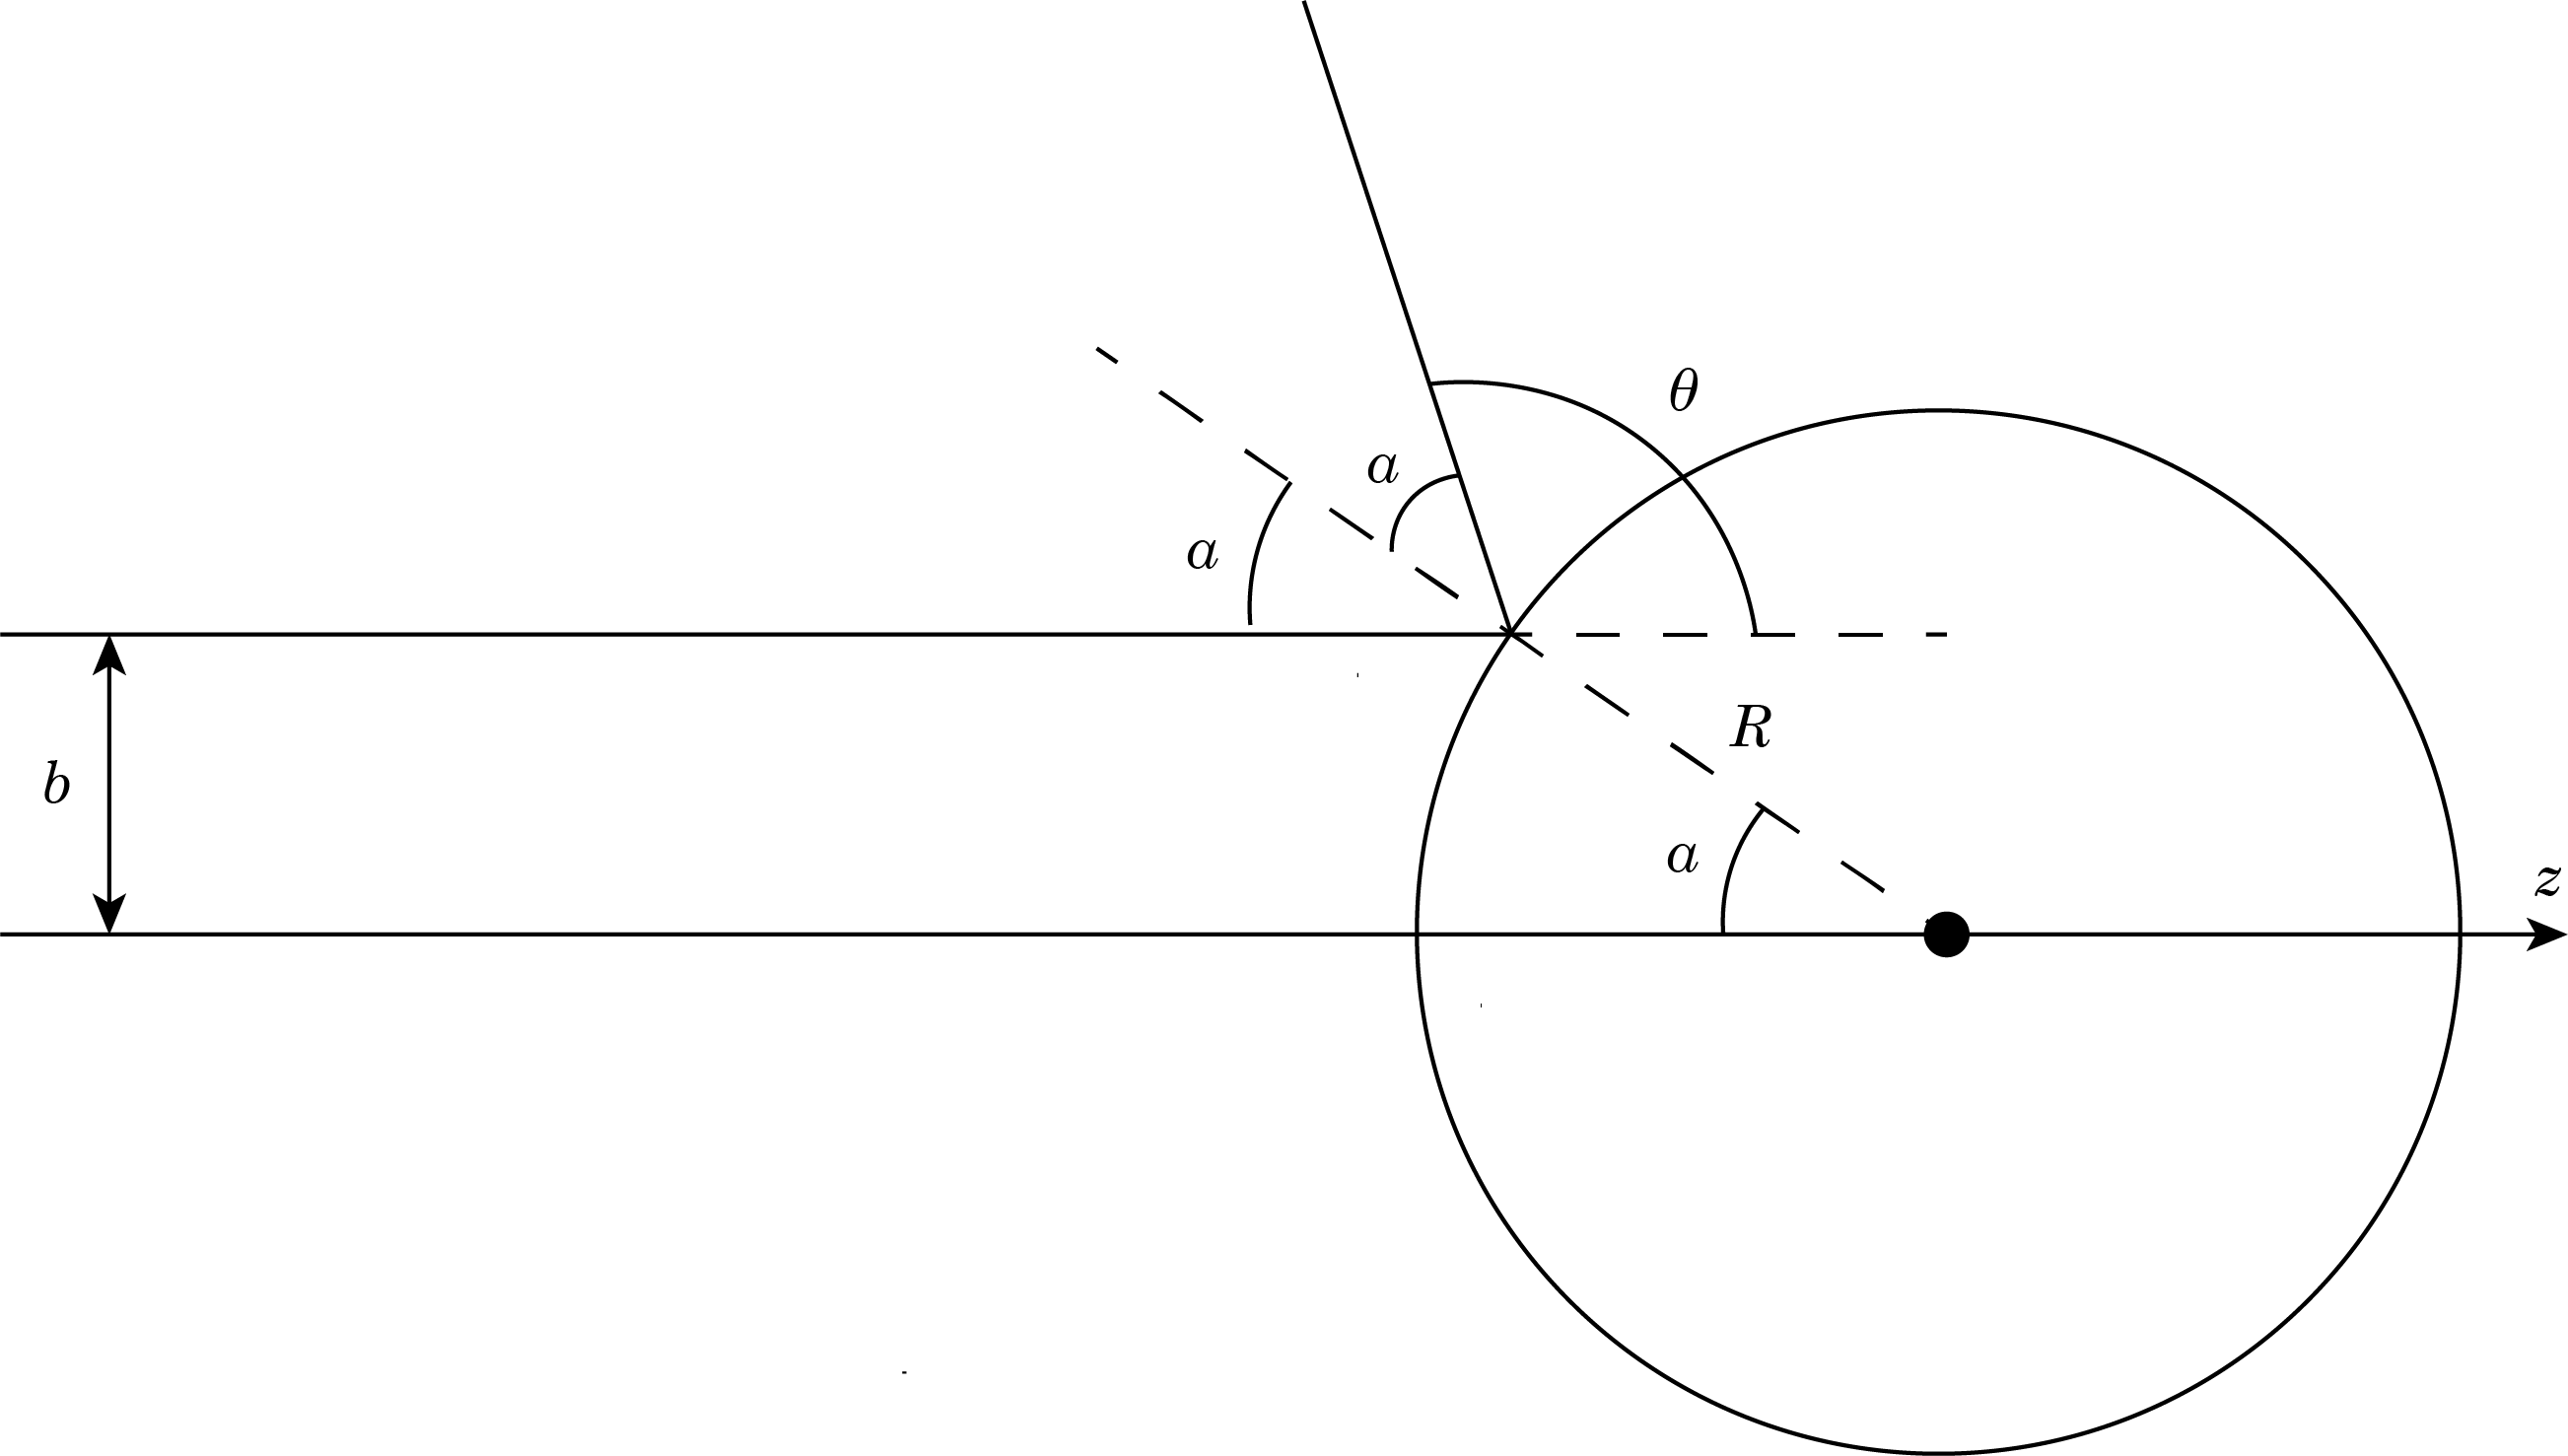
\includegraphics[scale=0.7]{class_4/images/2d-scattering-sphere.png}
\caption{Упругое рассеивание на жёсткой сфере в 2D}
\label{fig 3.1}
\end{figure}

Для примера можно рассмотреть упругое рассеивание на жесткой сфере. В 2D (рис. \ref{fig 3.1}) ситуация достаточно простая. Пусть сфера имеет радиус $R$. Тогда прицельный параметр равен $b = R\sin\alpha$, а угол рассеяния $\theta = \pi - 2\alpha$, где $\alpha$ -- угол между горизонталью и местом соприкосновения. Избавимся от этого угла и выразим $\theta$ через параметр $b$.
\begin{gather*}
b = R \sin\left(\frac{\pi}{2} - \frac{\theta}{2}\right) = R\cos\left(\frac{\theta}{2}\right)\\
\theta = \begin{cases} 2\arccos(b/R), & b \leq R, \\ 0,& b\geq R.\end{cases}
\end{gather*}

\begin{figure}[ht]
\centering
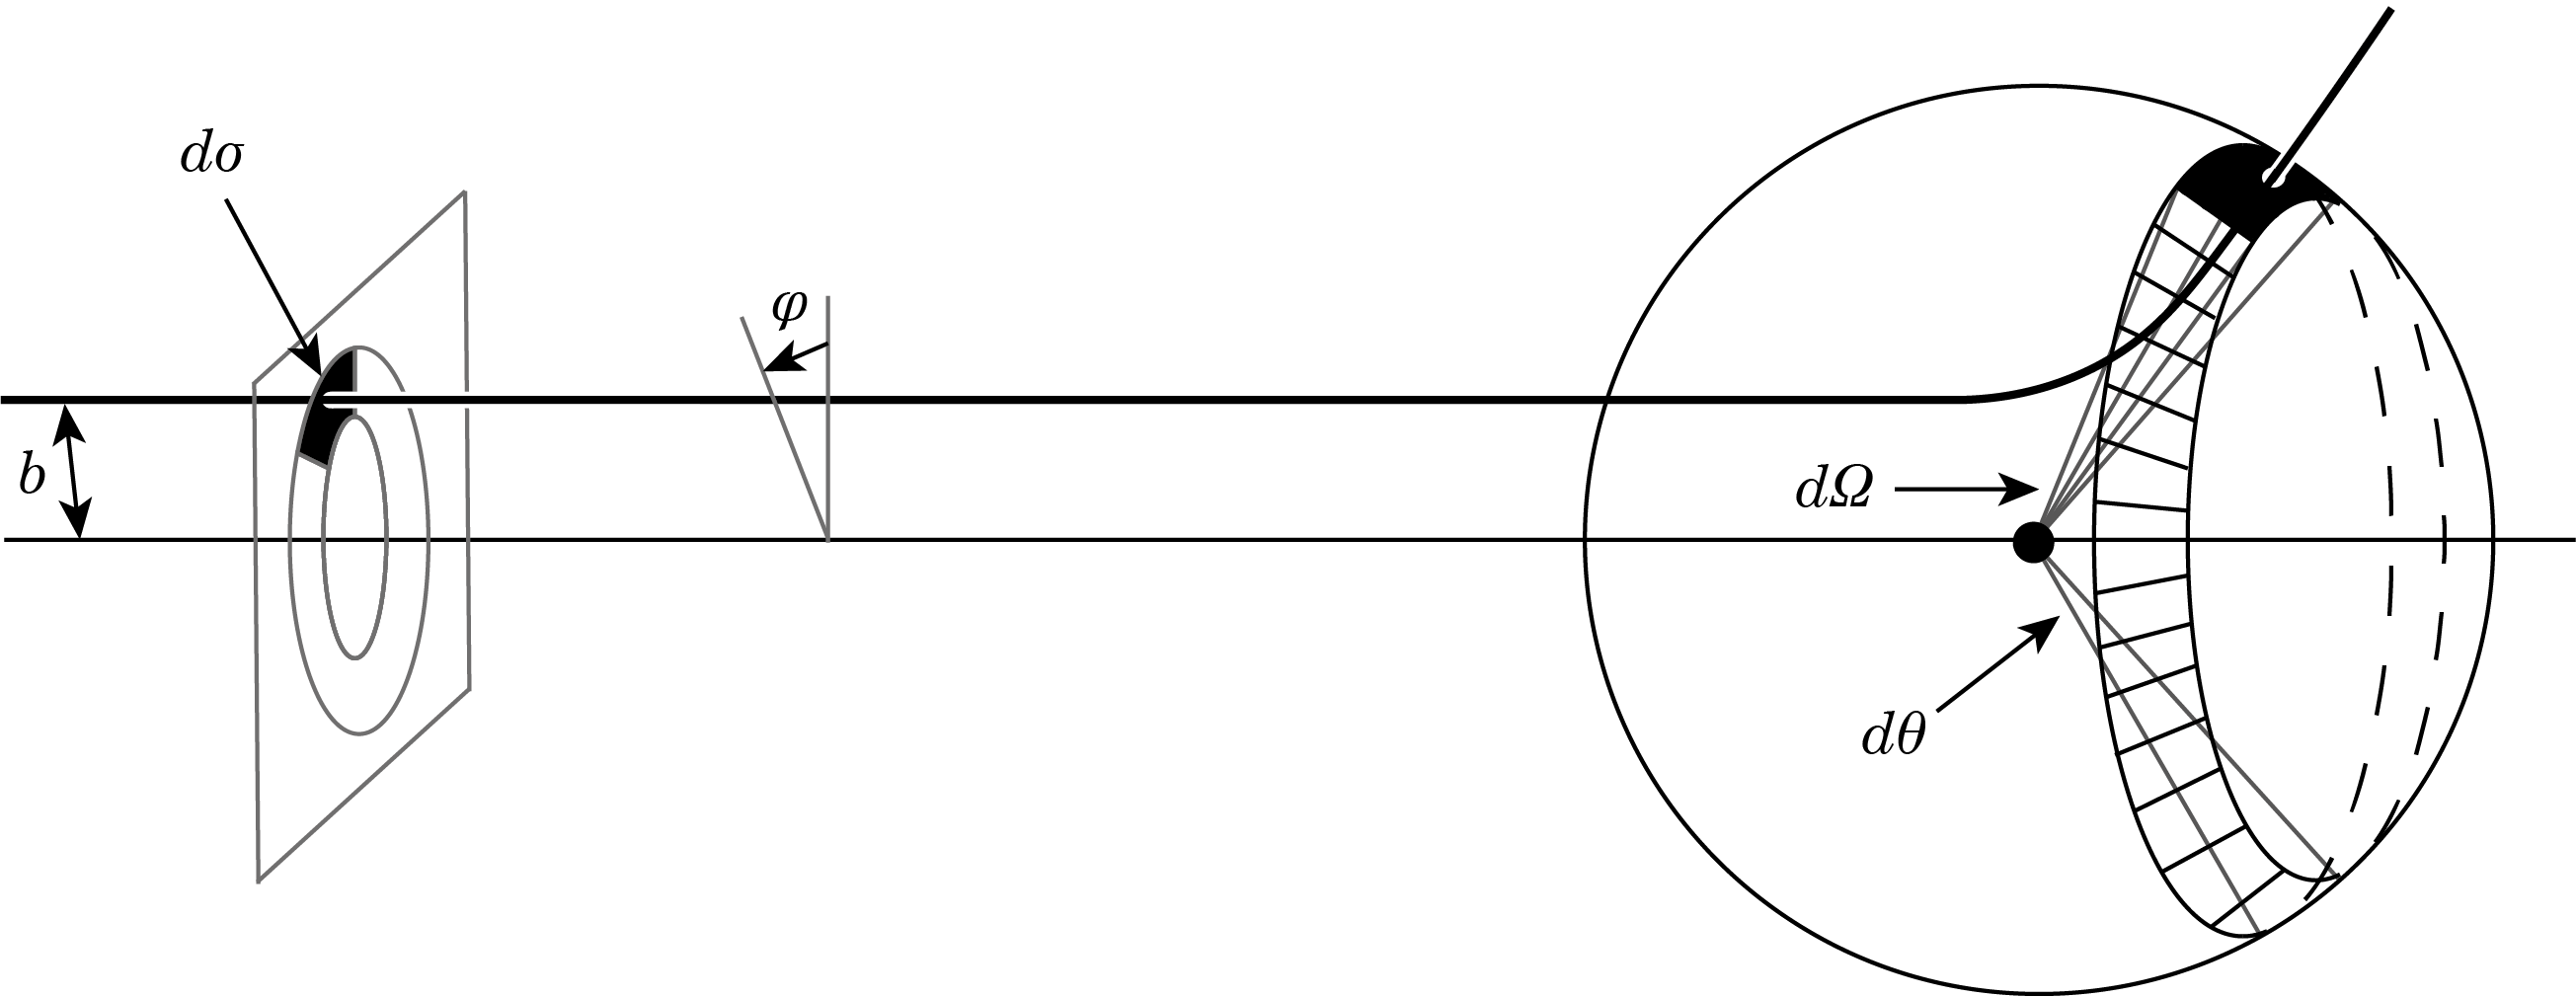
\includegraphics[scale=0.7]{class_4/images/3d-scattering-sphere.png}
\caption{Упругое рассеивание на жёсткой сфере в 3D}
\label{fig 3.2}
\end{figure}

В трехмерном случае для удобства введём несколько новых обозначений. Пусть $d\sigma$ -- элементарная область пролёта частиц, имеющая название эффективное сечение, а $d\Omega$ -- элементарная область, через которую пролетают частицы после рассеяния, называющаяся телесным углом. Чем больше $d\sigma$, тем больше $d\Omega$ -- их отношение выражает параметр $D(\theta) =d\sigma/d\Omega$. Он носит название дифференциальное эффективное сечение и в основном выражается следующим образом:
\[
d\sigma = D(\theta)d\Omega
\]

Если выразить всё через прицельный параметр $b$ и углы $\theta$ и $\phi$, где $\phi$ это азимутальный угол в сферической системе координат (рис. \ref{fig 3.2}), то эффективное сечение выражается как $d\sigma = b\,db\,d\phi$, а телесный угол $d\Omega = R^2\sin\theta\,d\theta\,d\phi$. Тогда, рассмотрев единичную сферу ($R=1$), получим следующее уравнение для дифференциального сечения рассеяния:
\[
D(\theta) = \frac{b}{\sin \theta}\left|\frac{db}{d\theta}\right|
\]

Рассмотрим ещё один способ выразить дифференциальное сечение рассеяния. Для этого введём величину $L$, отражающую количество частиц, проходящих через элементарную область за единицу времени. Тогда количество частиц, прошедших область $d\sigma$ за единицу времени выражается как $dN=L\,d\sigma$. Тогда, выражая $d\sigma$ через телесный угол, получим
\[
D(\theta) = \frac{1}{L}\frac{dN}{d\Omega}
\]
Такое выражение удобно в эксперименте, так как все параметры легко получить практически.

Используя оба варианта, мы можем получить полное сечение рассеяние. Оно выражается через интеграл дифференциального сечения рассеяния по всему телесному углу:
\[
\sigma = \int D(\theta)\,d\Omega
\]

\subsection{Квантовая теория рассеяния}
Для переформулировки теории рассеяния на ``квантовый язык'', нужно вспомнить, что частицы в квантовой механике обладают волновыми свойствами, а потому мы будем считать, что на рассеивающий потенциал налетает волна, которая затем образует сферический фронт с определенной амплитудой (по принципу Гюйгенса-Френеля). Тогда, запишем волновую функцию частицы как суперпозицию этих двух состояний:
\[
\psi(r,\,\theta)\approx A\left[e^{ikz} + f(\theta)\frac{e^{ikr}}{r}\right]
\]
Волновое число $k$ определяется так же, как и в первом семестре, связывая волновую функцию с энергией:
\[
k \equiv \frac{\sqrt{2mE}}{\hbar}
\]

Действительно важным в этом определении оказывается амплитуда рассеяния $f(\theta)$, так как именно она будет определять вероятность рассеяния на определенный угол $\theta$ и, соответственно, будет связана с дифференциальным сечением рассеяния. Действительно, посмотрим на вероятность квантовой частицы пролететь через площадь $d\sigma$ со скоростью $v$ за время $dt$:
\[
dP = |\psi|^2\, dV = |A|^2(v\, dt)\,d\sigma
\]
С другой стороны, можно выразить вероятность, что частица пройдет через соответствующий телесный угол $d\Omega$:
\[
dP = |\psi|^2\,dV = \frac{|A|^2|f(\theta)|^2}{r^2}(v\,dt)r^2\,d\Omega
\]
Тогда, сравнения эти выражения, получим что $d\sigma = |f(\theta)|^2\,d\Omega$, или другими словами
\[
D(\theta) = |f(\theta)|^2
\]
В итоге большинство задач рассеяния сводится к нахождению амплитуды рассеяния $f(\theta)$. Далее мы рассмотрим два популярных подхода для подсчёта $f(\theta)$: анализ парциальных волн (partial wave analysis) и аппроксимацию Борна.
\subsubsection{Метод парциальных волн}
Давайте аккуратно раскроем формализм этого подхода. Для этого вспомним, что в случае симметричного сферического потенциала волновая функция разделяется на радиальную и угловую, то есть $\psi(r,\,\theta,\,\phi) = R(r)Y^{m}_l(\theta,\,\phi)$. Напомню, что $Y^{m}_l(\theta,\,\phi)$ это сферические гармоники, а $u(r) = rR(r)$ должно удовлетворять радиальному уравнению:
\[
-\frac{\hbar^2}{2m}\frac{d^2u}{dr^2} + \left[V(r) + \frac{\hbar^2}{2m}\frac{l(l+1)}{r^2}\right]u = Eu
\]

\begin{figure}[ht]
\centering
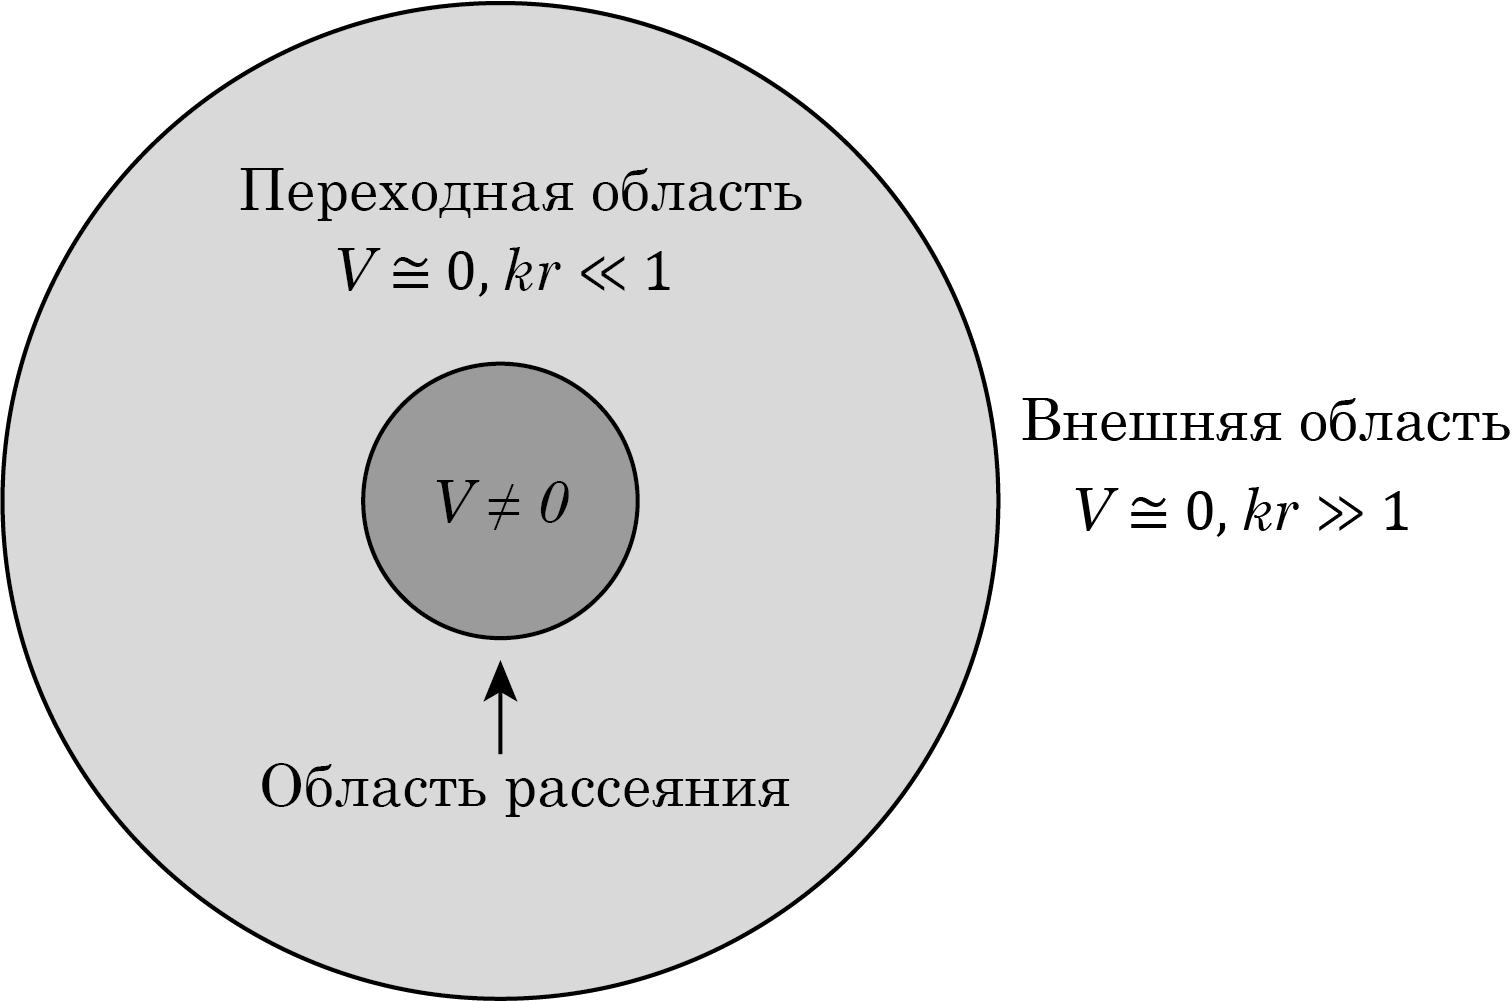
\includegraphics[scale=0.8]{class_4/images/localized-potential.png}
\caption{Локализованная модель потенциала, содержащая область рассеяния ($V\neq 0$), переходную область ($V\simeq 0,\, kr\ll 1$) и внешнюю область ($V\simeq 0,\, kr\gg 1$)}
\label{fig 3.3}
\end{figure}

Рассмотрим локализованную модель (рис. \ref{fig 3.3}). Идея парциального метода состоит в том, чтобы, используя граничные условия между переходной областью и областью рассеяния, найти амплитуду рассеяния. Для этого нужно определить, как выглядит волновая функция вне внутренней области.

Начнём с простого случая -- рассмотрим внешнюю область, где $r$ очень большая. Тогда оба члена, стоящие в скобках в радиальном уравнении можно не учитывать. Получим уравнение
\[
\frac{d^2u}{dr^2}\approx - k^2u,
\]
для которого мы знаем общее решение
\[
u(r) = Ce^{ikr} + De^{-ikr}
\]
Первый член это исходящая волна, второй же -- входящая. Для задачи рассеяния мы не хотим рассматривать входящие волны, поэтому $D=0$. В таком случае, для большого $r$ получаем что
\[
R(r) \sim \frac{e^{ikr}}{r}
\]

Теперь рассмотрим ситуацию в переходной области, когда мы не можем выкинуть второй член в скобках в радиальном уравнении. Тогда получим
\[
\frac{d^2 u}{dr^2} - \frac{l(l+1)}{r^2}u = -k^2 u
\]
Это -- уравнение Бесселя. Мы с ним уже встречались в первой части в семинаре номер 10. Оно естественным образом возникает при решении задач со сферическими потенциалами, то есть как раз наш случай. Итак, решение для такого уравнения выглядит как линейная комбинация сферических функций Бесселя:
\[
u(r) = Ar\,j_l(kr) + Br\,n_l(kr)
\]
К сожалению, это решение нам не совсем подходит, так как функции Бесселя ведут себя почти как тригонометрические. Нам же нужна линейная комбинация функций, описывающих входящие и исходящие волны, то есть $e^{ikr}$ и $e^{-ikr}$. Такие функции называются сферическими функциями Ханкеля:
\[
h^{(1)}_l(x) \equiv j_l(x) + in_l(x);\quad h^{(2)}_l(x) \equiv j_l(x) - in_l(x).
\]
По той же причине, что и в случае с внешней областью, нам нужны только функции Ханкеля первого типа, так как именно они при больших $r$ ведут себя пропорционально $e^{ikr}/r$:
\[
R(r)\sim h^{(1)}_l(kr)
\]

Соединяя всё это, получим точную волновую функцию вне внутренней зоны:
\[
\psi(r,\,\theta,\,\phi) = A\left[e^{ikz} + \sum\limits_{l, m} C_{l,m} h^{(1)}_l(kr) Y^m_l (\theta,\,\phi)\right]
\]
Это уравнение нужно немного переработать. Для начала заметим, что мы рассматриваем сферическо-симметричный потенциал. Из этого следует, что сферически потенциал не может зависеть от $\phi$, то есть $m=0$. Тогда $Y^{0}_l(\theta,\, \phi) = \sqrt{(2l+1)/4\pi}\,P_l(\cos\theta)$, где $P_l$ это полиномы Лежандра. Тогда, определив коэффициенты как $C_{l,0} \equiv i^{l+1}k\sqrt{4\pi(2l+1)}a_l$, получим 
\[
\psi(r,\,\theta,\,\phi) = A\left[e^{ikz} + k\sum\limits_{l=0}^{\infty}i^{l+1}(2l+1)\,a_l\,h^{(1)}_l(kr) Y^m_l (\theta,\,\phi)\right]
\]
Коэффициенты $a_l$ называются \textit{парциальными амплитудами}, находя которые мы и будем определять амплитуду рассеяния.

Проблема этого уравнения в том, что оно содержит два члена, записанных в разных системах координат. Попробуем переписать член $e^{ikz}$ в сферических координатах. Для этого вспомним, что общее решение может быть записано как 
\[
\sum\limits_{l, m}\left[A_{l,m}\, j_l(kr) + B_{l, m} n_l(kr)\right]Y^{m}_{l}(\theta,\,\phi)
\]
То есть, член $e^{ikz}$ может быть записан в подобном виде. Учитывая, что $e^{ikz}$ конечное (начинается от источника), член $n_l(kr)$ необходимо занулить, так как он быстро растёт при $r\rightarrow 0$. Так же не будем забывать, что $m$ должно быть равно нулю, чтобы не было зависимости от угла $\phi$. Тогда, можем записать \textit{формулу Рэлея}
\[
e^{ikz} = \sum\limits_{l=0}^{\infty} i^{l}(2l+1)\,j_l(kr)P_l(\cos\theta)
\]
Подставив это в исходное уравнение, получим волновую функцию, полностью описываемую переменными $r$ и $\theta$:
\[
\psi(r,\,\theta) = A\sum\limits_{l=0}^{\infty}i^{l}(2l+1)\left[j_l(kr) + ik\,a_l \, h^{(1)}_l(kr)\right]P_l(\cos\theta)
\]

Выразим амплитуду рассеяния $f(\theta)$ через парциальные амплитуды $a_l$. Для этого рассмотрим волновую функцию при больших $r$. Тогда, так как функция Ханкеля ведёт себя как $(-i)^{l+1}e^{ikr}/r$, можно записать волновую функцию в изначальном виде
\[
\psi(r,\, \theta) \approx A\left[ e^{ikz} + f(\theta)\frac{e^{ikr}}{r}\right],
\]
где амплитуда рассеяния выражается как
\[
f(\theta) = \sum\limits_{l=0}^{\infty}(2l+1)\,a_l\,P_l(\cos\theta)
\]
Вычислив интеграл от $|f(\theta)|^2$, получим полное сечение рассеяния, выраженное через парциальные амплитуды:
\[
\sigma = 4\pi\sum_{l=0}^{\infty}(2l+1)|a_l|^2
\]

Теперь, мы имеем все необходимые инструменты на руках, чтобы можно было решать различные базовые задачи. Классическая стратегия их решения -- используя граничные условия, найти парциальные амплитуды $a_l$, решая уравнение Шрёдингера для области рассеяния. После этого мы легко можем получить амплитуду рассеяния или полное сечение. Проиллюстрируем это на задаче с рассеянием на жёсткой сфере с радиусом $a$. 

\exercise
Потенциал в этой задаче выглядит следующим образом:
\[
V(r) = \begin{cases}\infty, &r\leq a \\ 0, &r>a\end{cases}
\]
Граничные условия очевидны: $\psi(a,\, \theta) = 0$. Тогда, используя формулы выше, получим уравнение на $a_l$:
\[
\sum\limits_{l=0}^{\infty}i^{l}(2l+1)\left[j_l(kr) + ik\,a_l \, h^{(1)}_l(kr)\right]P_l(\cos\theta) = 0
\]
Из этого уравнения выразим $a_l$:
\[
a_l = i\frac{j_l(ka)}{k\,h^{(1)}_l(ka)}
\]
Тогда, полное сечение будет выглядеть следующим образом:
\[
\sigma = \frac{4\pi}{k^2}\sum\limits_{l=0}^{\infty}(2l+1)\left|\frac{j_l(ka)}{h^{(1)}_l(ka)}\right|^2
\]

Понимаю, сама по себе это формула может не вызывать в вас какие-то возвышенные чувства, возбуждение или даже искреннюю радость. Всё-таки, это точное решение, которое нам часто мало интересно. Рассмотрим лучше случай $ka\leq 1$, который физический можно интерпретировать как малость сферы относительно длины волны рассеиваемой частицы. Тогда, так как для маленьких $ka$ функция $j_l(ka)$ сильно меньше, чем $n_k(ka)$, проведём следующие преобразования:
\[
    \frac{j_{l}(ka)}{h^{(1)}_{l}(ka)} = \frac{j_{l}(ka)}{j_{l}(ka) + i\,n_l(ka)} \approx -i\frac{j_{l}(ka)}{n_{l}(ka)} \approx i\frac{2^l l!\,z^l}{(2l+1)!}\frac{2^l l!}{(2l)!z^{-l-1}} = \frac{i}{2l+1}\left[\frac{2^l l!}{(2l)!}\right]^2 z^{2l+1}
\]
Подставляя это в полное сечение, получим:
\[
\sigma \approx \frac{4\pi}{k^2}\sum\limits_{l=0}^{\infty}\frac{1}{2l+1} \left[\frac{2^ll!}{(2l)!}^4\right] (ka)^{4l+2}
\]
Всё ещё выглядит не очень. Давайте учтём, что $ka \ll 1$, поэтому доминирующий член будет при $l=0$. Тогда оказывается, что 
\[
\sigma \approx 4\pi a^2
\]
Это может звучать не логично, потому что срез сферы -- это круг, соответственно должно быть $\pi a^2$. Но оказывается, что в квантовой механике и в оптике полное сечение будет равно полной площади сферы. Это один из примеров, показывающий отличие квантовой теории рассеяния от классической.
\csquare{darklavender}
\subsection{Сдвиг фазы}
\hspace{1.35em} Хоть мы уже и упростили задачу рассеяния, нам этого не достаточно. Вместо того чтобы искать комплексные числа, мы хотим искать вещественные. В этой части семинара будет описан метод, как реализовать такой переход. Основан он будет на поиске \textit{сдвига фазы} $\delta$.

Проиллюстрирую на наглядном примере. Пусть в одномерной задаче имеется рассеивающий локализованный потенциал с радиусом действия $a$ (рис. \ref{fig 3.4}). Поставим прямо за ним (в точку $x=0$) стену, от которой волна будет отражаться полностью. Тогда волновая функция вне зоны взаимодействия потенциала ($x < -a$) будет описываться падающей волной $\psi(x) = Ae^{ikx}$ и отраженной $\psi(x) = Be^{-ikx + \phi}$. Так как вся волна должна была отразиться, модули амплитуд должны сохраниться, то есть $|A| = |B|$, но фаза совсем не обязательно.

\begin{figure}[ht]
\centering
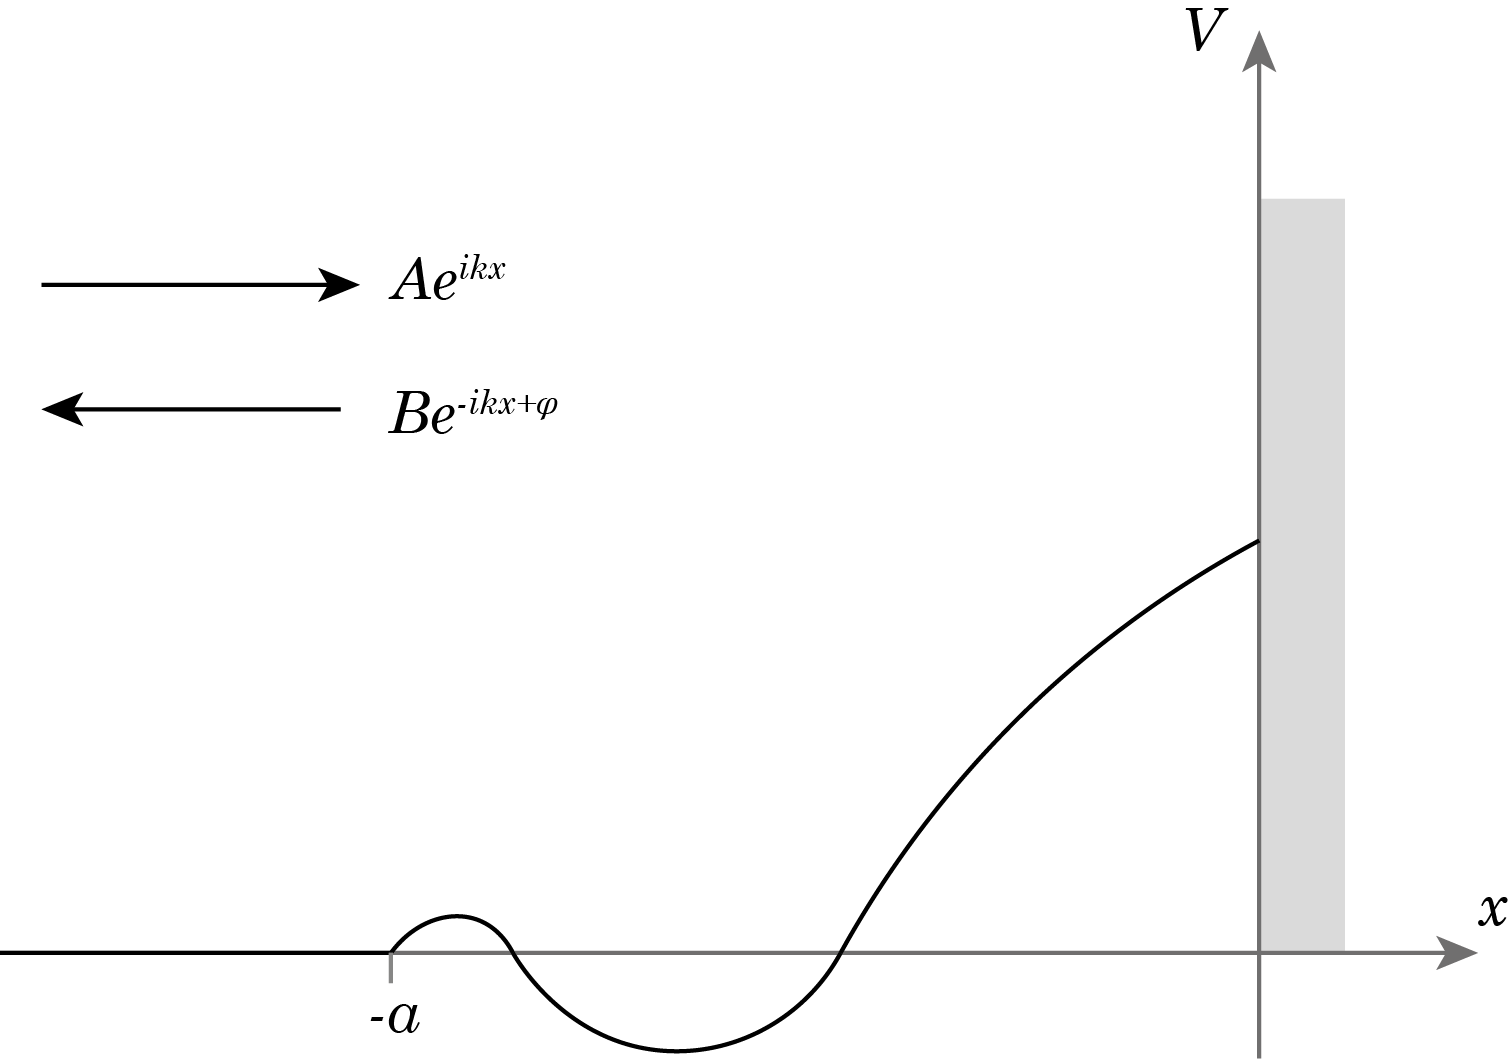
\includegraphics[scale=0.7]{class_4/images/one-dim-potential.png}
\caption{Одномерная модель произвольного рассеивающего потенциала с отражающей стеной в центре}
\label{fig 3.4}
\end{figure}

Пусть потенциал равен нулю, то есть взаимодействия нет, только отражающая стена. Тогда полная волновая функция выглядит следующим образом
\[
\psi(x) = A(e^{ikx} + e^{-ikx}),\quad (V=0)
\]
Если потенциал не нулевой, под его действием на отраженную волну может набежать фаза $\delta$. Тогда волновая функция преобразуется и получится:
\[
\psi(x) = A(e^{ikx} + e^{-ikx + i2\delta}),\quad (V\neq0)
\]
Коэффициент 2 перед сдвигом фазы это скорее соглашение. Его идея в том, что потенциал подействовал на волну два раза: один раз когда она шла к потенциалу, другой раз когда шла от него.

Теперь для решения задачи о рассеянии достаточно найти сдвиг фазы $\delta$ для конкретного потенциала. Это делается аналогично поиску парциальных амплитуд -- необходимо решить уравнение Шрёдингера в области рассеяния и применить правильные граничные условия. Проделав всё необходимое, мы получим вещественное число $\delta$ вместо комплексного $a_l$, которое содержит в себе точно такое же количество информации.

Вы можете возразить, сказав, что обычно мы работаем не в одномерии, поэтому этот подход не применим в реальном мире. Я приму это возражение серьезно и предложу рассмотреть ситуацию в 3D. В этом случае работает полученная выше формула Рэлея, которая не содержит $m$, но содержит всё возможные угловые моменты $l=0, 1,\dots$. Так как мы потенциал сферический, угловой момент сохраняется -- значит каждая парциальная волна рассеивается независимо, и изменения у неё происходят только в фазе. Таким образом мы можем переформулировать полученную формулу для парциальных амплитуд $a_l$ через фазовый сдвиг $\delta_l$. 

Рассмотрим ситуацию, когда потенциала нет, то есть $V(r)=0$. Тогда $\psi = Ae^{ikz}$, то есть
\[
\psi^{(l)} = Ai^{l}(2l+1)j_l(kr)P_l(\cos \theta)
\]
Используя аппроксимацию для больших $r$, получим
\[
j_{l}(x)\approx\frac{1}{2x}\left[ (-i)^{l+1} e^{ix} + i^{l+1} e^{-ix} \right]
\]
и подставим это приближение в волновую функцию
\[
\psi^{(l)} \approx A\frac{(2l+1)}{2ikr}\left[ e^{ikr} - (-1)^l e^{-ikr} \right] P_l(\cos\theta)
\]

Теперь необходимо добавить потенциал. Он повлияет на выражение выше следующим образом: второй член в скобках отвечает за сферическую волну, полученную из исходящей волны, поэтому она остаётся неизменной. Первый же член отвечает за сферическую волну, полученную из входящей волны и потенциал будет влиять на неё -- к ней добавится сдвиг по фазе:
\[
\psi^{(l)} \approx A\frac{(2l+1)}{2ikr}\left[ e^{i(kr+2\delta_l)} - (-1)^l e^{-ikr} \right] P_l(\cos\theta)
\]
Остаётся найти связь предыдущего подхода, основанного на парциальных волнах, со сдвигом фазы. Для этого выпишем уравнение в парциальных волнах для большого $r$ и сравним с уравнением, полученным выше:
\[
\psi^{(l)} \approx A\frac{(2l + 1)}{r}\left[ \frac{1}{2ik} \left(e^{ikr} - (-1)^l e^{-ikr}\right) + a_l e^{ikr} \right]
\]
Сравнивая эти уравнения, выразим $a_l$ через сдвиг фаз:
\[
a_l = \frac{1}{2ik}\left(e^{2i\delta_l} - 1\right) = \frac{1}{k}e^{i\delta_l}\sin(\delta_l)
\]
Тогда амплитуду и полное сечение рассеяния можно переписать через сдвиг фаз:
\begin{gather*}
    f(\theta) = \frac{1}{k}\sum_{l=0}^{\infty}(2l+1)e^{i\delta_l}\sin(\delta_l)P_l(\cos\theta)\\
    \sigma = \frac{4\pi}{k^2}\sum_{l=0}^{\infty}(2l+1)\sin^2(\delta_l)
\end{gather*}
Подводя итоги, можно сказать, что такой подход с использованием сдвига фаз помогает проще интерпретировать задачу физически и математически, так как мы уменьшаем количество вещественных значений с двух у комплексных $a_l$ до одного $\delta_l$. И магии здесь нет -- мы просто используем тот факт, что угловой момент сохраняется. Пример задач на поиск сдвига фазы смотрите в семинаре №6.

В следующем семинаре мы посмотрим на ещё один подход для решения задач рассеяния, называемый аппроксимацией Борна. 